\documentclass[11pt]{article}
\usepackage[a4paper,margin=0.82in,headheight=22pt,footskip=26pt]{geometry}
\usepackage[T1]{fontenc}\usepackage[utf8]{inputenc}\usepackage{lmodern}\usepackage{microtype}
\usepackage{amsmath,amssymb,amsthm,mathtools,bm}\usepackage{graphicx}
\usepackage{booktabs,tabularx,longtable,array,multirow}\usepackage{enumitem}\usepackage{xcolor}
\usepackage[most]{tcolorbox}\usepackage{titlesec}\usepackage{fancyhdr}\usepackage{caption,subcaption}
\usepackage{float}\usepackage{natbib}\usepackage{hyperref}\usepackage{url}\usepackage{setspace}\usepackage{placeins}
\definecolor{ink}{HTML}{203A56}\definecolor{teal}{HTML}{247C78}\definecolor{coral}{HTML}{C65F4B}\definecolor{pale}{HTML}{EEF4F7}\definecolor{muted}{HTML}{5B6873}
\hypersetup{colorlinks=true,linkcolor=ink,citecolor=teal,urlcolor=teal,pdfauthor={Devanik Debnath},pdftitle={The Hodge Obstruction to Escape-Proof Therapy}}
\setstretch{1.12}\setlength{\parindent}{1.15em}\setlength{\parskip}{0.28em}
\setlist[itemize]{leftmargin=1.45em,itemsep=0.15em,topsep=0.2em}\setlist[enumerate]{leftmargin=1.55em,itemsep=0.15em,topsep=0.2em}
\titleformat{\section}{\Large\bfseries\color{ink}}{\thesection}{0.65em}{}\titleformat{\subsection}{\large\bfseries\color{teal}}{\thesubsection}{0.6em}{}
\titlespacing*{\section}{0pt}{1.65em}{0.55em}\titlespacing*{\subsection}{0pt}{1.15em}{0.35em}
\pagestyle{fancy}\fancyhf{}\fancyhead[L]{\small\color{muted}HODGE OBSTRUCTION}\fancyhead[R]{\small\color{muted}PREPRINT \textbullet{} 25 OCT 2026}\fancyfoot[C]{\small\color{muted}\thepage}
\renewcommand{\headrulewidth}{0.4pt}\renewcommand{\headrule}{\hbox to\headwidth{\color{teal}\leaders\hrule height \headrulewidth\hfill}}
\newtheorem{proposition}{Proposition}[section]\newtheorem{theorem}[proposition]{Theorem}\newtheorem{lemma}[proposition]{Lemma}
\theoremstyle{definition}\newtheorem{definition}[proposition]{Definition}\theoremstyle{remark}\newtheorem{remark}[proposition]{Remark}
\newtcolorbox{keybox}{colback=pale,colframe=teal,boxrule=0.8pt,arc=2mm,left=2.5mm,right=2.5mm,top=1.5mm,bottom=1.5mm}
\newtcolorbox{caveatbox}{colback=white,colframe=coral,boxrule=0.8pt,arc=2mm,left=2.5mm,right=2.5mm,top=1.5mm,bottom=1.5mm}
\newcommand{\R}{\mathbb{R}}\newcommand{\V}{\mathcal{V}}\newcommand{\A}{\mathcal{A}}\newcommand{\Ssafe}{\mathcal{S}}\newcommand{\Rrisk}{\mathcal{R}}\newcommand{\Kviab}{\mathcal{K}}\newcommand{\E}{\mathbb{E}}\newcommand{\Prob}{\mathbb{P}}\newcommand{\ind}{\mathbf{1}}
\title{\vspace{-1.1cm}{\Huge\bfseries\color{ink}The Hodge Obstruction to Escape-Proof Therapy}\\[0.45em]{\large\color{muted}A structural no-go result, a robust safety game, and a reproducible synthetic benchmark for drug-sequence design}}
\author{Devanik Debnath\\[-0.1em]\small Department of Electronics and Communication Engineering\\\small National Institute of Technology Agartala, India\\\small ORCID: \href{https://orcid.org/0009-0001-8310-6921}{0009-0001-8310-6921} \quad GitHub: \href{https://github.com/Devanik21}{Devanik21}}
\date{25 October 2026 \quad $\vert$ \quad Theoretical and synthetic-computational preprint v1.0.0}
\begin{document}\maketitle
\begin{abstract}
Drug-sequence design seeks to steer evolving pathogen populations away from states that support multi-drug resistance. A tempting topological hypothesis is that a Hodge decomposition of drug-specific collateral-effect fields reveals a curl or harmonic obstruction to a schedule that remains safe indefinitely. This paper subjects that hypothesis to a structural test before using it as a design principle. If, for each drug, an edge effect is defined as the difference of a single scalar fitness potential at the two endpoint genotypes, then the edge field is exact: its circulation around every closed path is zero by telescoping, and its square-face curl vanishes identically. On the complete cubical complex, the first cohomology also vanishes. Therefore, nonzero curl cannot be a structural property of a consistent static scalar fitness landscape; it instead signals noisy or incomplete measurements, a mismatched field definition, or genuinely state- and history-dependent dynamics. Hodge analysis remains useful as a data-consistency diagnostic, but it does not by itself decide whether escape-proof therapy exists. We then formulate escape avoidance as a finite-state robust safety game and prove that its greatest fixed point is the exact viability kernel for a specified successor relation. A finite-horizon probabilistic dynamic program and tabular Q-learning baseline are compared on a reproducible, four-locus, three-landscape synthetic benchmark. The synthetic result is intentionally modest: a robustly safe subset exists for the declared toy rules, while one-step greedy and round-robin policies enter the synthetic failure set frequently in seeded simulations. These numbers are not antimicrobial measurements and support no clinical recommendation. The paper's contribution is a falsifiable separation principle: audit the measured edge field with Hodge tools, but establish safety with reachability and viability analysis under explicit mutation and observation assumptions.
\end{abstract}
\noindent\textbf{Keywords:} antimicrobial resistance; evolutionary game theory; combinatorial Hodge decomposition; viability kernel; partial observation; drug sequencing; synthetic benchmark; reinforcement learning.
\begin{keybox}\textbf{Core conclusion.} A consistent scalar fitness landscape produces an exact edge field with zero cycle circulation. A therapy schedule is escape-proof only relative to a specified transition model, failure set, observation model, and adversary—not because a Hodge component happens to be nonzero.\end{keybox}
\begin{caveatbox}\textbf{Scope and status.} This is a theory-plus-synthetic-simulation preprint. Numerical landscapes are generated by the released code; no pathogen-specific dataset, wet-lab experiment, patient data, or clinical protocol was used. The proposed safety-game framework is not a treatment recommendation.\end{caveatbox}
\tableofcontents\clearpage\label{maintext-start}

\section{Introduction: from drug sequences to safety guarantees}
Antimicrobial resistance is an evolutionary control problem with an asymmetric objective. A sequence may temporarily suppress growth yet leave the population in a genetic background from which cross-resistance is easier to reach. Empirical and model-based work has therefore investigated sequential drug use as a way to steer evolutionary trajectories, rather than treating each drug as an isolated intervention. Studies of collateral sensitivity show both the potential of sequencing and its dependence on evolutionary repeatability: the same first drug may lead different replicates to different genetic endpoints, changing their response to a later drug \citep{Nichol2019,MaltasWood2019,ArdellKryazhimskiy2021}. A recent reinforcement-learning study demonstrates that treatment cycling policies can be learned over empirically measured landscapes in silico despite noisy or delayed observations \citep{Weaver2024}. These are important precedents, not evidence that a universal escape-proof schedule exists.

The question here is more stringent than minimizing average growth. Let genotype be a vertex of a finite mutation graph, let a drug be an action, and let the transition model describe which mutations can follow that action. Mark a subset of vertices as failure states—for example, genotypes above declared resistance thresholds for multiple drugs. Does there exist a policy that keeps the trajectory outside that set for all future time, despite allowed mutation outcomes and incomplete information? This is a safety-game question. Its answer depends on the transition relation, the failure set, and what the controller can observe.

The proposed title invokes a Hodge obstruction because topological summaries of edge flows can distinguish gradient, local-circulation, and harmonic components. Combinatorial Hodge methods have a well-developed mathematical foundation and have been applied to biological structures and data analysis \citep{Jiang2011,Koh2022}. The critical issue is whether the particular edge field in drug-sequence design is actually a non-conservative flow. When it is constructed from differences of a scalar fitness landscape, the answer is no: the field is a discrete gradient by definition. The paper makes that logical constraint explicit and redirects topology from a purported cause of therapeutic impossibility to an audit of data coherence.

\begin{figure}[htbp]\centering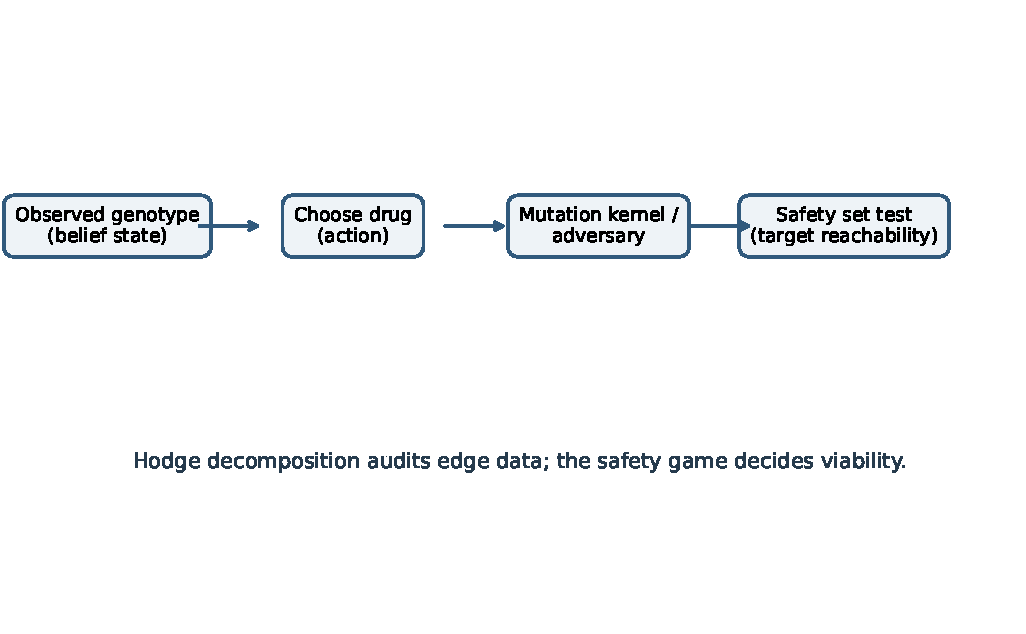
\includegraphics[width=0.92\linewidth]{figures/fig01_framework.pdf}\caption{Workflow separation. Hodge decomposition audits edge-field consistency; the robust safety game addresses whether a policy can remain inside a declared safe set. Conceptual diagram, not an empirical result.}\label{fig:framework}\end{figure}

The deliverable is a set of definitions, two finite-state results, and a small executable benchmark. The structural result rules out one interpretation of the conjecture under its own assumptions. The safety-game theorem supplies the correct object for an escape guarantee: the greatest controlled-invariant subset of the safe region. A finite-horizon stochastic counterpart quantifies risk when transitions are not treated adversarially. The synthetic example demonstrates why a static landscape summary and a control guarantee answer different questions.

\section{Research posture and claim classification}
We treat the initial Hodge-obstruction conjecture as a hypothesis to be falsified, not a desired conclusion. The manuscript distinguishes exact mathematics from modeled dynamics and synthetic outputs. An algebraic identity on a hypercube is not a claim that a pathogen follows a hypercube in full biological detail. A viability result is conditional on the transition relation used to compute it. The benchmark is deliberately small enough that exact dynamic programming and robust fixed-point computation can be independently checked.

The contribution has three parts. First, it provides a no-go statement: when every drug-specific edge field is the exact difference of a scalar node potential, its closed-loop circulation must vanish. Second, it states a finite-state safety-game characterization of infinite-horizon escape avoidance and makes the partial-observation extension explicit. Third, it provides a reproducible toy benchmark that exercises the distinction between exact Hodge structure, noisy edge measurements, adversarial viability, finite-horizon risk, and a learned policy. These elements are a synthesis and formalization of existing ingredients; this search does not establish priority for a new field of evolutionary therapy or a new general Hodge theorem.

\begin{table}[htbp]\centering\small\caption{Claim classification and evidential status.}\label{tab:claims}\begin{tabularx}{\linewidth}{p{0.30\linewidth}p{0.15\linewidth}X}\toprule Claim & Class & Status and limitation\\\midrule Scalar-potential edge differences have zero loop sum & P1 & Exact telescoping identity on any finite graph.\\ Hodge decomposition separates exact, coexact, and harmonic components & P1 & Standard finite-dimensional decomposition; depends on oriented complex and inner product.\\ A greatest-fixed-point kernel characterizes robust perpetual safety & P1/P2 & Exact for a finite, fully specified controlled transition relation.\\ The synthetic model contains a nonempty robust safe subset & Model-dependent & Verified by code for the declared toy landscapes and successor relation.\\ Real pathogen therapy can be made escape-proof by a Hodge score & Unsupported & Not established; this paper rejects the inference.\\\bottomrule\end{tabularx}\end{table}

\section{Related work and the actual gap}
\subsection{Evolution on measured fitness landscapes}
Mira and colleagues measured adaptive landscapes for TEM $\beta$-lactamase genotypes across multiple antibiotics and concentration conditions, supporting combinatorially complete analyses of a small mutational system \citep{Mira2015}. Nichol et al. used landscape structure to demonstrate that collateral sensitivity can be contingent on the trajectory generated under the first treatment, rather than being a deterministic mapping from one drug to the next \citep{Nichol2019}. Maltas and Wood analyzed diverse collateral-sensitivity profiles and optimal sequencing strategies, including laboratory population experiments \citep{MaltasWood2019}. Ardell and Kryazhimskiy developed a population-genetic theory for collateral resistance and sensitivity \citep{ArdellKryazhimskiy2021}. Together these studies motivate trajectory-level planning and warn against assuming all replicates follow a single path.

A measured finite landscape does not automatically define an escape-proof policy. It supplies phenotype or fitness values for genotypes under specified conditions; it does not by itself determine a universally correct mutation kernel. Mutation rates, fixation probabilities, population size, drug concentration, spatial structure, and observation noise may change which transitions are feasible or likely. Mira et al. specifically showed that adaptive landscape structure depends on antibiotic concentration, reinforcing the need to state environmental conditions rather than treat fitness values as immutable properties \citep{Mira2015}.

\subsection{Optimal control and reinforcement learning}
Nichol et al. modelled sequential therapy as a biased random walk on fitness landscapes and analyzed how drug order changes the emergence of resistance \citep{Nichol2015}. Weaver et al. used empirically parameterized landscapes and reinforcement learning to learn drug cycling policies under partial, noisy, or delayed information; they compared learned strategies with exact optimization and simpler cycling policies \citep{Weaver2024}. Therefore, the broad idea of using RL to optimize drug sequences is not new and is not claimed as this paper's novelty. Here, tabular Q-learning is a transparent baseline; it is not a clinical agent and does not certify worst-case safety.

\subsection{Hodge decomposition and fitness data}
Combinatorial Hodge theory decomposes edge flows into gradient-like, curl-like, and harmonic components when an appropriate simplicial or cubical complex is specified. Jiang et al. developed HodgeRank for ranking from pairwise comparisons, where cyclic inconsistency is a meaningful property of observed comparisons \citep{Jiang2011}. Wei et al. applied Hodge tools to biomolecular structure and biological data represented by simplicial complexes \citep{Koh2022}. These works support the mathematical legitimacy of a Hodge audit; they do not imply that every biological edge field is non-conservative or that its Hodge components determine policy viability.

\subsection{The defensible gap}
The narrow gap addressed here is not the general use of Hodge decomposition in biology, nor drug scheduling via reinforcement learning. It is the need to separate (i) consistency diagnostics for measured edge effects from (ii) robust reachability guarantees under an explicit drug-controlled transition relation. We could not establish absolute novelty from targeted searches, and adjacent work is extensive. The specific contribution is a no-go correction to the proposed interpretation plus a reproducible safety-game formulation. Table~\ref{tab:literature} contrasts research roles.

\begin{table}[htbp]\centering\small\caption{Closest prior work and the limited position of the present paper.}\label{tab:literature}\begin{tabularx}{\linewidth}{p{0.27\linewidth}p{0.36\linewidth}X}\toprule Work & Established contribution & Relationship here\\\midrule Mira et al. (2015) & Empirical TEM $\beta$-lactamase landscapes; environment-dependent fitness & Motivates scalar landscapes; no data are reused in the synthetic runs.\\ Nichol et al. (2019) & Path-dependent collateral responses and replicate heterogeneity & Motivates explicit transition/path modeling.\\ Maltas and Wood (2019) & Collateral sensitivity profiles and sequence optimization & Prior landscape-based sequencing; no claim of replacing it.\\ Weaver et al. (2024) & RL treatment cycling with imperfect observations & Clarifies that RL-for-sequencing already exists.\\ Jiang et al. (2011); Wei et al. (2022) & Combinatorial Hodge theory and biological applications & Establishes Hodge tools; present focus is exactness of scalar fitness differences.\\ This preprint & No-go separation plus robust finite-state safety characterization & Synthetic mathematical illustration only; no new empirical therapy.\\\bottomrule\end{tabularx}\end{table}

\section{Genotype complex, landscapes, and orientation}
Let $G=(V,E)$ be a finite, connected mutation graph. A vertex $x\in V$ represents a genotype or coarse-grained genetic state; an undirected edge connects genotypes one allowed mutation apart. For a four-locus binary example, $V=\{0,1\}^4$ has 16 vertices and 32 edges. We consider $m$ candidate drugs/actions indexed by $a\in\A=\{1,\ldots,m\}$. Under fixed assay conditions, drug $a$ is represented by a scalar landscape $f_a:V\to\R$.

Orient each edge arbitrarily. For oriented edge $e=(u,v)$, define the drug-specific edge cochain
\begin{equation}\label{eq:edge}\omega_a(e)=f_a(v)-f_a(u).\end{equation}
Reversing orientation changes the sign. This is the discrete analogue of a gradient field. It represents a fitness difference only when both endpoint values are measurements of the same landscape under the same environmental and assay definition. It is not the same object as a mutation probability, transition log-odds, or policy-dependent average velocity.

Epistasis does not invalidate Eq.~\eqref{eq:edge}. Epistasis changes the values of $f_a$ on vertices, but the differences still telescope as long as a single-valued landscape is used. Multiple drugs may have different and opposing gradients; each $\omega_a$ remains exact separately. Switching environments creates a nonautonomous controlled process, but it does not make each drug's static edge field non-exact.

\begin{figure}[htbp]\centering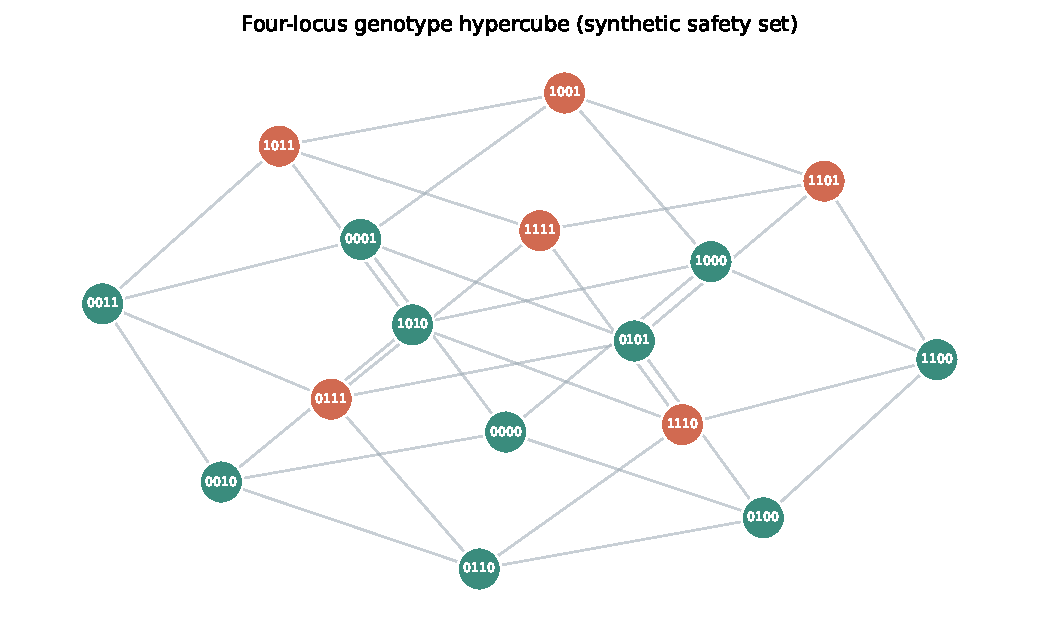
\includegraphics[width=0.84\linewidth]{figures/fig02_genotype_hypercube.pdf}\caption{The 4-locus hypercube used in the synthetic example. Labels are bit strings. Orange vertices satisfy the illustrative failure criterion; teal vertices do not. All assignments are model-generated.}\label{fig:cube}\end{figure}

\section{A Hodge no-go proposition for scalar fitness gradients}
Let $B_0\in\R^{|E|\times |V|}$ be the oriented edge-vertex incidence operator with row $e=(u,v)$ containing $-1$ at $u$ and $+1$ at $v$. Then the edge cochain in Eq.~\eqref{eq:edge} is $\omega_a=B_0f_a$. Let $B_2\in\R^{|F_2|\times |E|}$ encode oriented boundaries of 2-faces in a cubical complex, with each row representing the signed cycle around a square. The square circulation is $B_2\omega_a$.

\begin{proposition}[Exactness forces zero circulation]\label{prop:exact}
For every scalar landscape $f_a:V\to\R$ and every directed cycle $C=(v_0,v_1,\ldots,v_k=v_0)$ whose edge effects are defined by Eq.~\eqref{eq:edge},
\begin{equation}\label{eq:telescoping}\sum_{i=0}^{k-1}\omega_a(v_i,v_{i+1})=0.\end{equation}
In particular, $B_2B_0=0$ and every square-face curl of $\omega_a$ vanishes exactly, up to numerical representation error.
\end{proposition}
\begin{proof}
Substituting the definition yields $\sum_{i=0}^{k-1}[f_a(v_{i+1})-f_a(v_i)]$. Every intermediate value appears once with each sign, leaving $f_a(v_k)-f_a(v_0)=0$. The square-face identity is a special case. In matrix terms, the boundary of a boundary vanishes, so $B_2B_0=0$.
\end{proof}

The result assumes neither additivity nor absence of epistasis, and it requires no distribution for mutational effects. It assumes only that the edge value is generated from one single-valued node potential. If edges are estimated independently from noisy assays, measured differences need not be consistent with a common potential. That departure may reveal uncertainty, assay mismatch, omitted covariates, or history dependence. It is not an intrinsic nonzero curl of the scalar potential assumed in the model.

\begin{figure}[htbp]\centering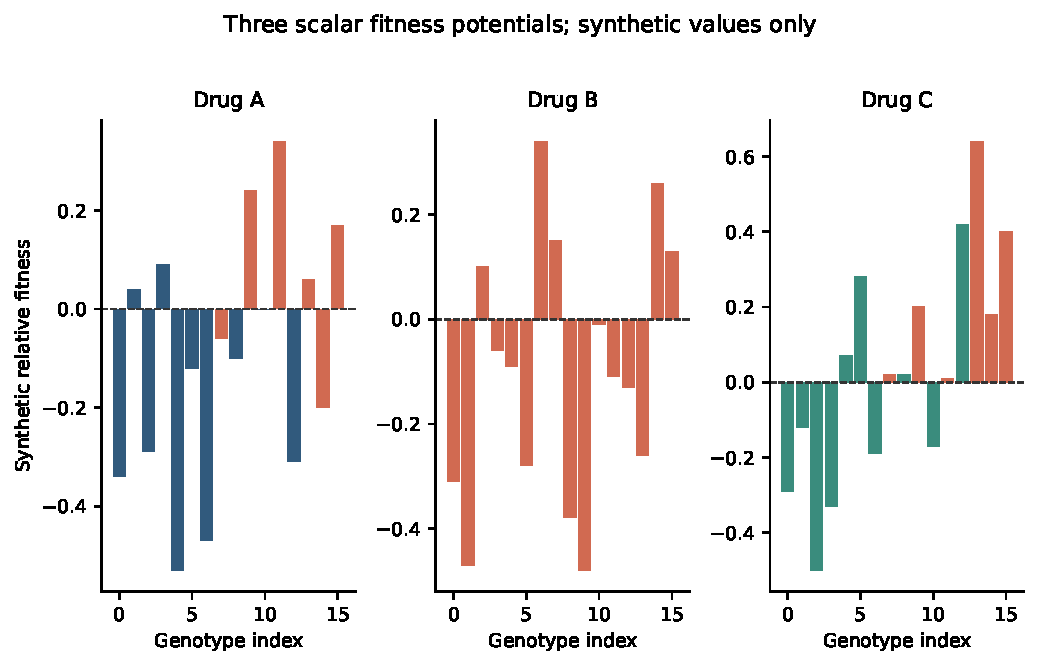
\includegraphics[width=0.90\linewidth]{figures/fig03_fitness_potentials.pdf}\caption{Three synthetic scalar fitness potentials over 16 genotype vertices. The dashed line is the illustrative threshold used in the toy failure-set definition, not a clinical breakpoint.}\label{fig:fitness}\end{figure}

\section{Hodge decomposition: what it can and cannot tell us}
For a finite oriented 2-complex, a 1-cochain $w\in\R^{|E|}$ may be decomposed orthogonally, under the Euclidean inner product, into exact, coexact, and harmonic components:
\begin{equation}\label{eq:hodge}w=B_0f+B_2^{\top}\phi+h,\qquad h\in\ker(B_0^{\top})\cap\ker(B_2).\end{equation}
The exact part captures edge differences induced by node scores; the coexact part captures local circulation represented by oriented 2-faces; and the harmonic part captures cycle structure not explained by those local faces. Precise operator naming depends on whether boundary or coboundary operators are used and how the complex is oriented, but the finite-dimensional orthogonal decomposition is standard \citep{Jiang2011,Koh2022}.

For the complete cubical complex of a hypercube, all faces are filled and the complex is contractible. Its first cohomology is trivial. Thus any exact edge field has no coexact or harmonic energy in exact arithmetic. Figure~\ref{fig:hodge} visualizes energy fractions from numerical projections of exact synthetic edge fields. The plotted floating-point residuals are machine-level artifacts, not biological signals. When independent noise is added to edge observations, apparent circulation becomes nonzero (Fig.~\ref{fig:curl}); this demonstrates a consistency diagnostic rather than a new evolutionary mechanism.

\begin{figure}[htbp]\centering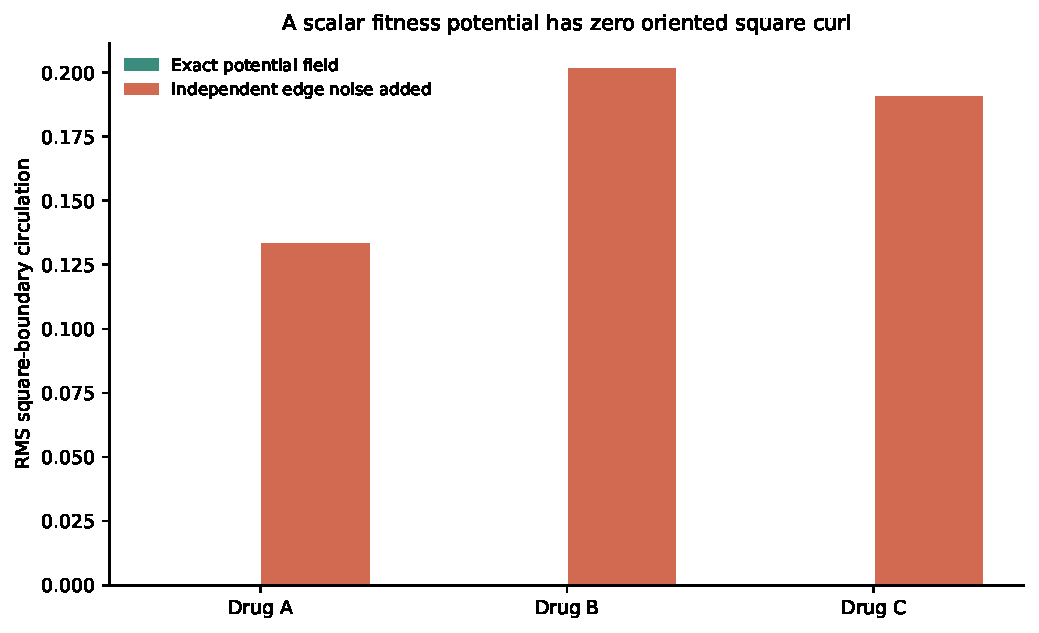
\includegraphics[width=0.86\linewidth]{figures/fig04_curl_exact_vs_noisy.pdf}\caption{RMS square circulation for exact scalar-potential differences versus fields with seeded independent edge noise. Exact circulation is at floating-point precision; noisy circulation reflects the synthetic error model.}\label{fig:curl}\end{figure}
\begin{figure}[htbp]\centering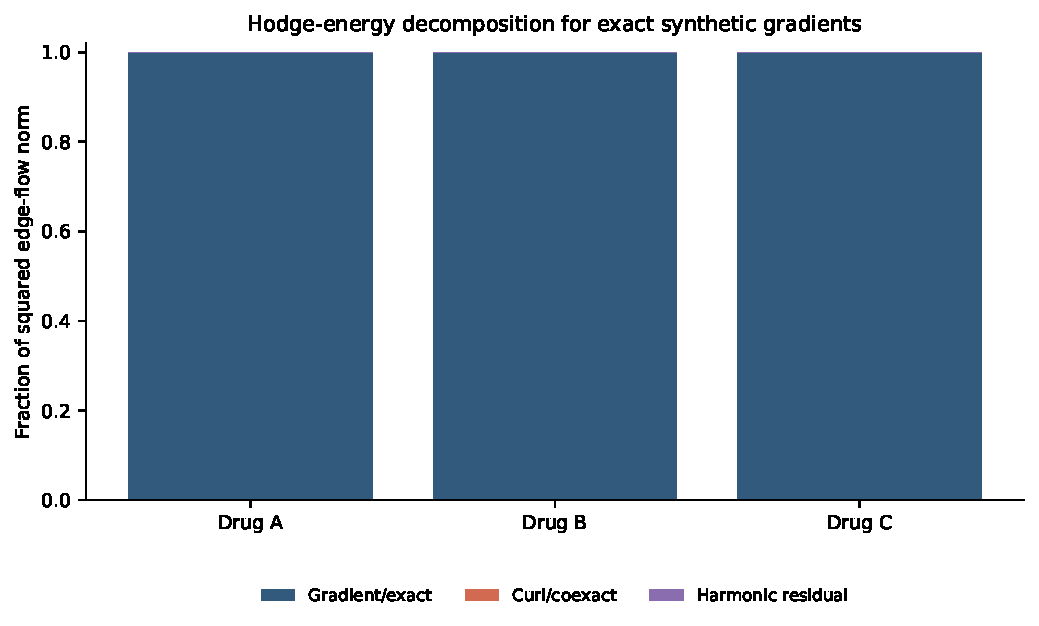
\includegraphics[width=0.86\linewidth]{figures/fig05_hodge_energy.pdf}\caption{Energy fractions after orthogonal projection of exact synthetic gradients onto gradient, coexact, and residual harmonic subspaces. Non-gradient fractions at numerical tolerance are not interpreted as real structure.}\label{fig:hodge}\end{figure}

\begin{proposition}[No Hodge-curl lower bound on drug count from static potentials]\label{prop:nolower}
Under the assumptions of Proposition~\ref{prop:exact}, the square-curl of each drug-specific landscape is identically zero regardless of the number of available drugs. Therefore, a nonzero static-landscape curl cannot yield a nontrivial lower bound on the number of drugs required for safety.
\end{proposition}
\begin{proof}
Apply Proposition~\ref{prop:exact} to every $f_a$. The result is zero for every action and does not depend on $m$. A lower bound on $m$ must arise from the transition relation, failure set, resource constraints, or partial observability—not from a quantity fixed at zero by the model definition.
\end{proof}

\section{What apparent curl might mean}
An observed circulation statistic remains worth reporting when carefully defined. We separate four cases. (i) If edge data were obtained by subtracting common, noise-free node scores, nonzero circulation indicates implementation or orientation error. (ii) If each edge effect was independently estimated with uncertainty, nonzero circulation can arise from measurement noise; the inference should quantify its scale. (iii) If the measured variable is not a fitness difference—such as a directional transition log-odds—it may legitimately be non-conservative, but its interpretation differs from a scalar fitness gradient. (iv) If fitness depends on hidden state, time, drug history, concentration, population composition, or spatial environment, a single static potential may be inadequate. The model then needs those state variables or must treat the field as an approximation.

Figure~\ref{fig:mutationgraph} shows the genotype adjacency graph with edges that can be beneficial in at least one synthetic drug environment highlighted. The graph is an accessibility scaffold, not a full probability model. It shows why the same vertices can support different directional transitions under different landscapes. It does not contradict exactness of each landscape's fitness differential: direction depends on which drug is active.

\begin{figure}[htbp]\centering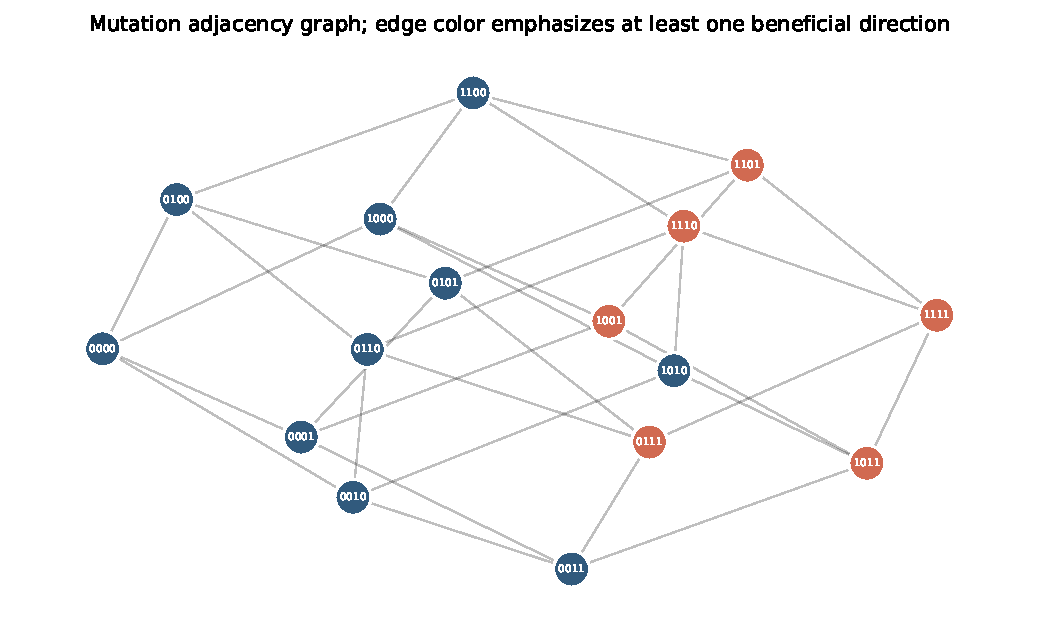
\includegraphics[width=0.83\linewidth]{figures/fig06_accessible_mutation_graph.pdf}\caption{Mutation adjacency graph. Teal edges have a beneficial direction under at least one synthetic drug. The graph summarizes accessibility; the actual successor relation is action-specific.}\label{fig:mutationgraph}\end{figure}

A nonzero curl could become mechanistically meaningful if a model explicitly defines a non-gradient edge field, for example from cyclic transition preferences or context-dependent dynamical observations. The empirical question is then whether that field predicts transitions or resistance outcomes beyond known fitness, mutational, and assay variables. A prospective test would fit the field on part of the data and assess calibration and predictive value on held-out trajectories. Without such evidence, “hysteresis-like” remains an analogy. History dependence requires comparing matched current genotypes after distinct randomized drug histories and observing whether transition distributions differ after controlling for measured confounders.

\section{Escape avoidance as a robust safety game}
Define a failure set $\Rrisk\subseteq V$ and a safe set $\Ssafe=V\setminus\Rrisk$. For each genotype $x$ and drug $a$, let $\mathrm{Succ}(x,a)\subseteq V$ be the set of possible one-step successors under the chosen model. A conservative strong-selection/weak-mutation stylization can include the current genotype and every one-mutation neighbor that is beneficial under drug $a$. In another application, it could be a confidence set for mutation transitions or an adversarial support set obtained from uncertain parameters.

The controller observes state $x$, chooses a drug $a$, and then nature or the evolutionary process selects any successor in $\mathrm{Succ}(x,a)$. The goal is to stay in $\Ssafe$ for all time. A policy is robustly safe from $x$ if every possible trajectory starting there avoids $\Rrisk$. This is intentionally stronger than a low average resistance probability. It provides a worst-case guarantee only relative to the declared successor relation; if that relation omits a biologically possible mutation, the guarantee does not cover it.

\begin{figure}[htbp]\centering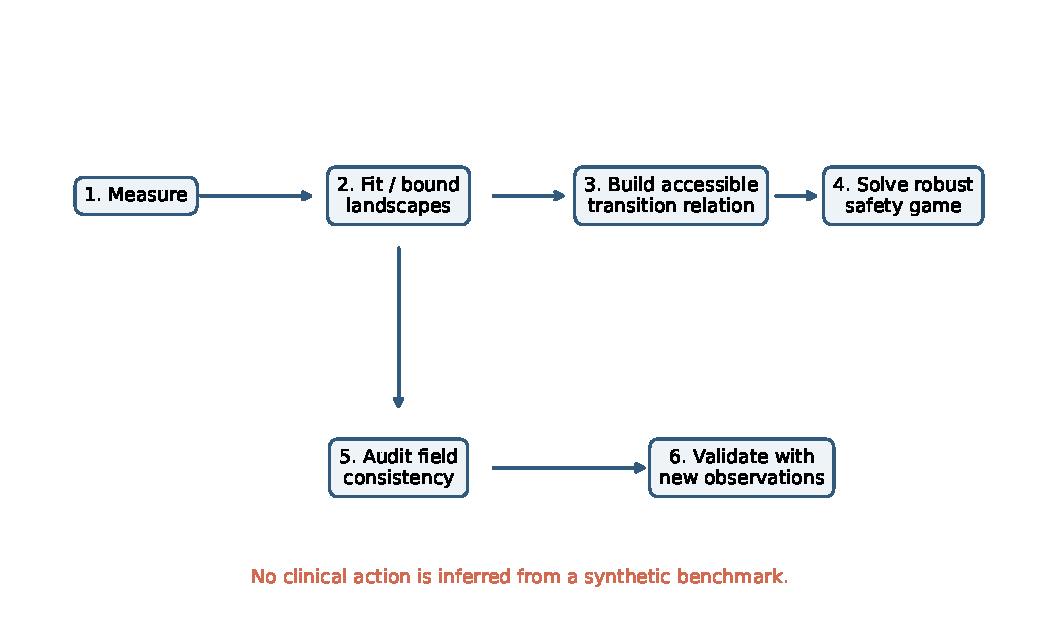
\includegraphics[width=0.86\linewidth]{figures/fig12_verification_workflow.pdf}\caption{Evidence-to-safety workflow. Measurement, transition modeling, robust synthesis, consistency auditing, and future validation remain distinct tasks. Procedural diagram only, not a clinical protocol.}\label{fig:workflow}\end{figure}

\section{Model uncertainty and robust-kernel sensitivity}
A controller may know the genotype but not the complete mutation support. Treating a guessed successor graph as exact can turn a numerical certificate into a false guarantee. Let $\mathfrak{T}$ be a set of admissible transition relations, each with successor set $\Gamma_T(x,a)$. The conservative predecessor operator is
\begin{equation}\label{eq:uncertainpre}
\operatorname{Pre}_{\mathfrak{T}}(K)=\{x\in K:\exists a\in\A(x),\ \forall T\in\mathfrak{T},\ \Gamma_T(x,a)\subseteq K\}.
\end{equation}
The robust kernel is the greatest fixed point obtained by starting at the declared safe set and iterating this operator. A state survives only if a single action works for every transition relation in the uncertainty family. This order of quantifiers is stronger than selecting an action separately after discovering which transition model is true.

\begin{proposition}[Monotonicity under transition uncertainty]
Suppose $\mathfrak{T}_1\subseteq\mathfrak{T}_2$ and both uncertainty families use the same state space, action availability, and safe set. Then their robust kernels satisfy $K_\infty(\mathfrak{T}_2)\subseteq K_\infty(\mathfrak{T}_1)$.
\end{proposition}
\noindent\textit{Proof.} For any candidate $K$, an action whose successors remain in $K$ for every $T\in\mathfrak{T}_2$ also does so for every $T\in\mathfrak{T}_1$, because the latter family contains no additional relation. Thus $\operatorname{Pre}_{\mathfrak{T}_2}(K)\subseteq\operatorname{Pre}_{\mathfrak{T}_1}(K)$. Both iterations begin at the same safe set. Induction gives inclusion at every iteration, and taking the finite fixed-point limits preserves inclusion. $\square$

This result is elementary but operationally important: enlarging a defensible uncertainty set can only preserve or shrink the certified region. It cannot improve a worst-case guarantee. Empirical use should therefore report how the kernel changes when plausible mutation edges, compensatory transitions, drug-specific observations, or unmeasured genotypes are added. A large kernel under an artificially sparse graph is not persuasive evidence of robust treatment design.

For measured landscapes, uncertainty can enter at two different layers. Fitness uncertainty changes the estimated direction or probability of an edge; transition uncertainty changes which edges are possible at all. The first can be represented by intervals or posterior distributions over potential differences. The second is a support question. A model that assigns tiny probability to an observed escape route has not eliminated that route from a robust game. In contrast, a finite-horizon expected-risk objective may legitimately weight it by probability, provided the calibration and loss function are justified.

An appropriate diagnostic should distinguish three statuses: certified safe under all declared transitions, low-risk under a calibrated probabilistic model, and unresolved because the measurement/transition support is incomplete. Collapsing those into a single “escape-free score” would hide the principal assumptions on which the conclusion depends.

\section{The viability kernel and an exact theorem}
For a subset $Q\subseteq\Ssafe$, define the controlled robust predecessor
\begin{equation}\label{eq:pre}\mathrm{Pre}(Q)=\{x\in\Ssafe:\exists a\in\A,\ \mathrm{Succ}(x,a)\subseteq Q\}.\end{equation}
Let $K_0=\Ssafe$ and recursively set $K_{n+1}=\mathrm{Pre}(K_n)$. The sequence is decreasing: a state is removed whenever every action admits at least one possible successor already excluded. Because $V$ is finite, the sequence stabilizes in at most $|V|$ strict reductions. Its fixed point is the robust viability kernel.

\begin{theorem}[Finite-state robust viability characterization]\label{thm:viability}
Let $V$ and $\A$ be finite and let $\mathrm{Succ}(x,a)$ be nonempty for every state-action pair. The limit $\Kviab=\bigcap_{n\ge0}K_n$ is exactly the set of states from which a policy can guarantee $x_t\in\Ssafe$ for every $t\ge0$ against every successor allowed by $\mathrm{Succ}$. For every $x\in\Kviab$, at least one action witnesses robust invariance. For every $x\in\Ssafe\setminus\Kviab$, no policy can guarantee indefinite safety under the stated successor relation.
\end{theorem}
\begin{proof}
Since the sets are finite and decreasing, there is an index $N$ for which $K_{N+1}=K_N$. Write this set as $K$. By the fixed-point definition, for every $x\in K$ there exists an action $a$ such that all successors lie in $K$. Selecting such an action at every state in $K$ keeps the next state in $K$; induction proves safety at all future times.

Conversely, any state removed at iteration $n+1$ is either already unsafe or, for every action, has at least one successor outside $K_n$. An adversary can choose such a successor. By induction on the removal iteration, any state outside the fixed point admits a finite sequence of allowed adversarial responses that reaches the failure set. Thus no policy guarantees perpetual safety from that state. This is a finite-state reachability argument; it does not use Hodge decomposition.
\end{proof}

The fixed-point iteration for the synthetic benchmark is shown in Fig.~\ref{fig:kernel}. It reports the size of the candidate safe set after each elimination step, and the final kernel is stored in \url{results/summary.json}. A nonempty kernel means the toy rules admit a robustly safe region. It does not establish that such a region exists for a real pathogen or that a clinically feasible regimen can keep a population inside it.

\begin{figure}[htbp]\centering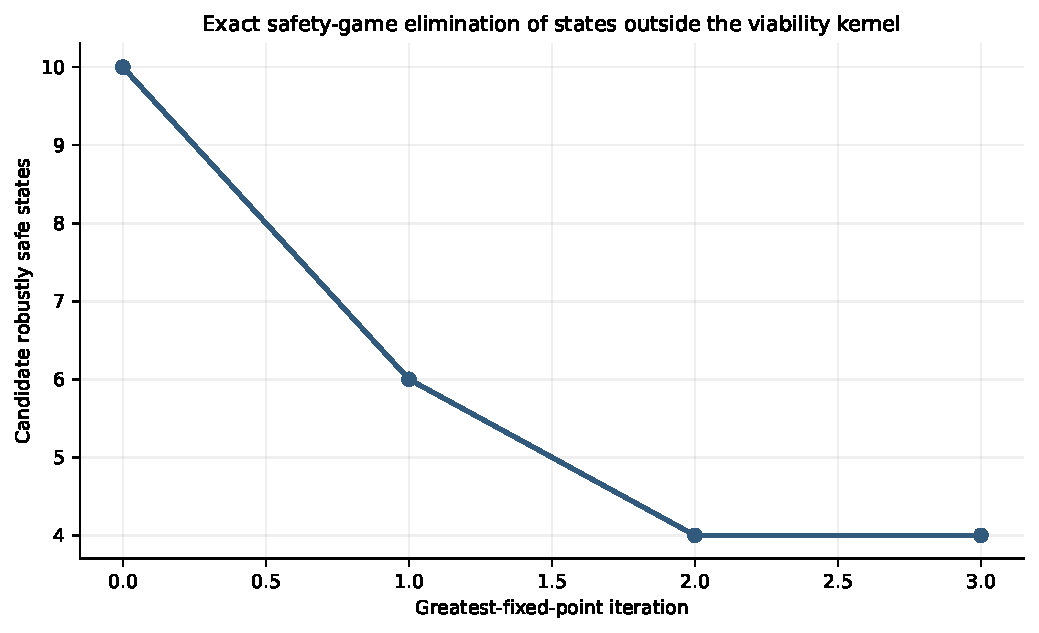
\includegraphics[width=0.82\linewidth]{figures/fig07_viability_kernel.pdf}\caption{Greatest-fixed-point iteration on the synthetic successor relation. Each iteration removes states without an action whose full successor set remains inside the previous candidate.}\label{fig:kernel}\end{figure}

\section{A probabilistic counterpart: finite-horizon risk}
Robust safety treats every allowed successor as an adversarial possibility. When a transition kernel is credible and the objective is probabilistic, define $P_a(x,y)$ as the probability of next genotype $y$ under action $a$. Let $J_h(x)$ be the minimum probability of entering $\Rrisk$ within the next $h$ transitions, with $J_0(x)=\ind_{\Rrisk}(x)$. Then
\begin{equation}\label{eq:dp}J_h(x)=\begin{cases}1,&x\in\Rrisk,\\ \min_{a\in\A}\sum_{y\in V}P_a(x,y)J_{h-1}(y),&x\in\Ssafe.\end{cases}\end{equation}
The minimizing action is horizon-dependent in general. This recursion is exact for the given finite-state Markov decision process and cost convention. It is not a robust guarantee, because a low-probability unmodeled event may still make escape possible. In the synthetic example, beneficial one-locus moves receive weights that increase exponentially with synthetic fitness difference, with a fixed stasis weight. This is a stress-test kernel, not a calibrated SSWM formula for an organism.

\begin{figure}[htbp]\centering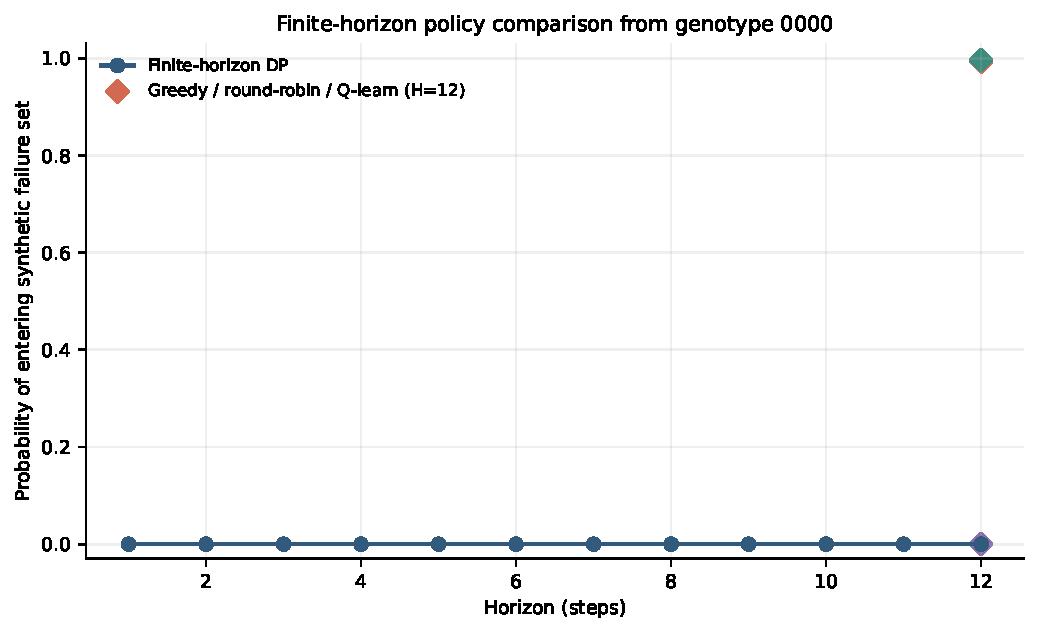
\includegraphics[width=0.83\linewidth]{figures/fig08_policy_risk_horizon.pdf}\caption{Finite-horizon policy comparison from genotype 0000. The exact DP curve and horizon-12 Monte Carlo estimates for simple and learned policies are synthetic. Dots are estimated over seeded trajectories, not clinical probabilities.}\label{fig:risk}\end{figure}

A practical decision maker may prefer expected growth suppression, cumulative hazard, time spent under ineffective therapy, drug toxicity, or switching costs rather than the probability of hitting $\Rrisk$ alone. These can be included as state-action costs, but should not be collapsed into an undocumented reward. The robust kernel and probabilistic DP answer different questions: the former asks whether every allowed transition can be kept safe; the latter asks how likely escape is under a probabilistic model and an optimizing policy.

\section{Partial observation and belief-state safety}
Sequencing does not always identify a single genotype. Measurements may be noisy, delayed, aggregated over a mixed population, or restricted to loci that do not distinguish relevant states. Let $b\subseteq V$ be the current belief support: all states compatible with the observation history. An action is robustly safe from belief $b$ only if every actual state in $b$ remains in the safe region and every possible successor and observation update preserves a safe belief. The belief transition is induced by both the hidden-state transition and the observation kernel.

For a set-valued abstraction, define $\mathrm{Post}(b,a)=\bigcup_{x\in b}\mathrm{Succ}(x,a)$. If observations are not used to refine state identity, a conservative belief predecessor is
\begin{equation}\label{eq:beliefpre}\mathrm{Pre}_{B}(Q)=\{b\subseteq\Ssafe:\exists a\in\A,\ \mathrm{Post}(b,a)\subseteq Q\}.\end{equation}
This set-based formulation can be conservative because it discards probabilities and the ability to distinguish outcomes. A more exact partially observed game augments the state with belief update, which can grow exponentially with $|V|$. On small landscapes, exact belief-state enumeration supplies a gold-standard comparator for approximate policies; on larger landscapes, interval bounds, abstraction refinement, or conformal sets for unseen genotype effects can control computational growth.

Figure~\ref{fig:matrix} maps the synthetic fitness values by action and genotype. The figure makes no claim that the numbers emulate empirical TEM data. It also highlights a limitation of point-estimate landscapes: a neural surrogate that fills unmeasured genotypes should return uncertainty or prediction sets, not only a single predicted fitness, if it is to support worst-case safety reasoning.

\begin{figure}[htbp]\centering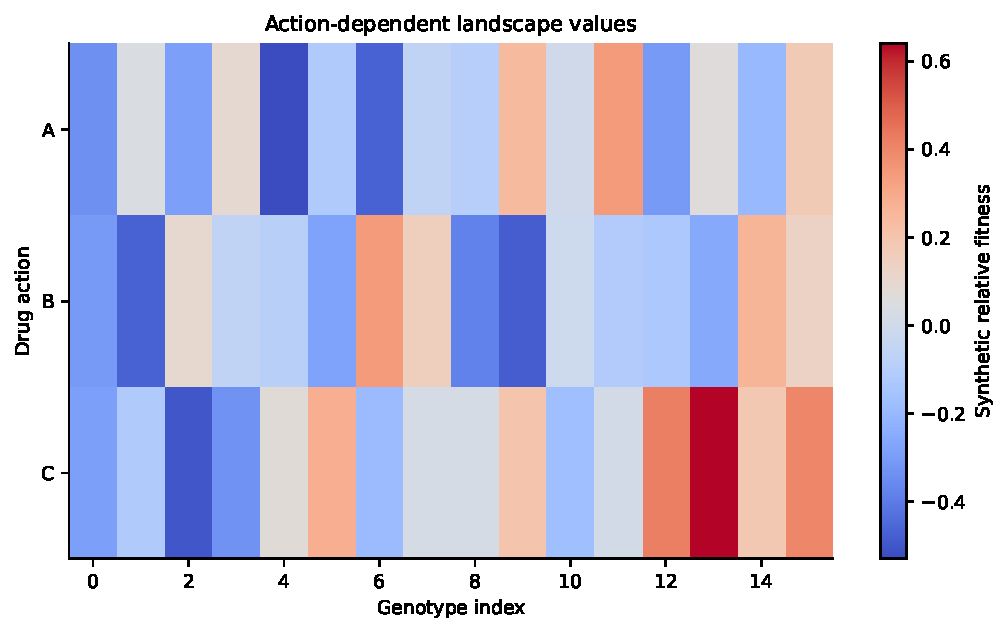
\includegraphics[width=0.76\linewidth]{figures/fig09_action_fitness_matrix.pdf}\caption{Synthetic action-by-genotype fitness matrix generated from the coefficients in the verification script. No bacterial measurements are included.}\label{fig:matrix}\end{figure}

\section{Estimating edge fields from noisy landscape measurements}
The exact-gradient result is most informative when it is turned into an estimable diagnostic. Suppose a noisy assay reports an oriented edge vector $y\in\mathbb{R}^{|E|}$ over a graph with incidence matrix $B$, where rows encode edge orientation. Under a static-potential null model, $y=Bf+\epsilon$, with latent vertex potential $f$ and measurement error $\epsilon$. Because adding a constant to every component of $f$ does not change $Bf$, estimation requires either a reference vertex or a gauge constraint such as $\mathbf{1}^{\top}f=0$ on each connected component.

For known positive precision weights $W$, the weighted least-squares estimate solves
\begin{equation}\label{eq:wls}
\widehat f=\arg\min_{f:\,\mathbf{1}^{\top}f=0}\lVert W^{1/2}(y-Bf)\rVert_2^2.
\end{equation}
The residual $r=y-B\widehat f$ measures the component that cannot be explained by a single potential under the chosen graph and weights. With the weighted inner product, the gradient projection is obtained from the corresponding normal equations. Cycle-space or Hodge projections provide an interpretable decomposition of this residual, but the residual is not automatically a biological hysteresis effect: finite-sample noise, assay batch effects, concentration drift, and omitted environmental covariates can all make independent edge observations fail to agree with a common scalar potential.

A test of the static-potential model therefore needs a measurement model, not just a plotted curl. Relevant checks include replicate-level variance, uncertainty-weighted residual norms, held-out edges, calibration across drug concentrations, and sensitivity to the cell complex used to define 2-faces. A graph with no filled 2-cells cannot test square-face closure, while adding a face is a scientific assumption about which cycle should be treated as a boundary. On a four-locus cube the face set is explicit; on an irregular empirical genotype graph, the appropriate complex may be uncertain.

If data are collected under multiple histories or environments, the null model should include those contexts as strata or covariates before residual circulation is interpreted. Matched genotypes may have distinct growth or transition responses after different prior drug exposures; that is a meaningful history-dependence hypothesis only when measurement, inoculum, growth phase, and assay context are controlled. If the apparent residual disappears under replication or context adjustment, the simpler noise explanation should be preferred.

Conversely, a stable residual on preregistered held-out cycles may motivate a richer state model. It still does not show that the residual decides whether a safe policy exists. The key empirical question is incremental utility: does a residual-derived feature improve calibrated prediction of held-out transitions or the performance of a safety policy relative to fitness differences, uncertainty bounds, and standard epistasis models? If not, the Hodge feature remains descriptive rather than a control-theoretic obstruction.

\section{A role for machine learning without confusing prediction and proof}
A learned landscape model can estimate $f_a(x)$ for unmeasured genotypes from sequence features, but its role is prediction. It does not, merely by fitting observed fitness, certify that its extrapolations preserve the true ranking or transition support. For safety analysis, an uncertainty-aware model should provide a set $\mathcal{F}_a(x)$ of plausible fitness values or a confidence bound. A conservative mutation relation then includes every transition possible under some landscape in the uncertainty set. The viability kernel computed with that enlarged relation is smaller than or equal to the kernel computed under a point estimate, because additional possible successors make robust control more difficult.

RL can be useful where the transition model is large, partially observed, or changes over time. However, reward optimization is not the same as a hard safety constraint. A Q-learning policy may obtain good average return while retaining nonzero probability of entering a failure state. A safe-RL formulation needs a shield or constraint mechanism based on a verified safe set, and the shield itself depends on the validity of the transition model. The prior Weaver et al. study already establishes the relevance of RL for treatment-cycle learning under imperfect observation in modeled landscapes \citep{Weaver2024}; this paper does not relabel that contribution as new.

\subsection{Synthetic Q-learning baseline}
The released code trains a tabular Q-learning policy for 9,000 episodes using the same finite genotype-state simulator and a penalty for entering the synthetic failure set. All episodes use deterministic random seeds for reproducibility. The learned policy is evaluated in independent 5,000-trajectory Monte Carlo runs. These choices permit a fair and inspectable software benchmark while remaining purposefully small. The policy is neither evidence of a general learning advantage nor a deployable antimicrobial treatment controller; its reward, transition model, and state representation are all stylized and fully known.

\section{Synthetic benchmark design}
The benchmark uses a 4-bit genotype hypercube with three scalar fitness landscapes. Landscape values are generated from a fixed intercept, four additive coefficients, and six pairwise interaction coefficients for each drug. These coefficients were selected as a transparent toy construction to create trade-offs and epistasis, not estimated from data. The failure set comprises states whose synthetic fitness meets the declared threshold under at least two of the three landscapes. In the released run, the threshold is zero in the dimensionless synthetic scale, yielding a finite nonempty failure set. This definition is internal to the example and must not be read as a resistance breakpoint.

For robust safety, a drug-specific successor set contains the current genotype and each one-locus neighbor with strictly greater synthetic fitness under that drug. The safety game assumes a worst-case selector chooses any member of this set after the drug is applied. For probabilistic risk, a separate transition matrix is formed by assigning a weight of one to stasis and a weight proportional to $\exp(\beta\Delta f)$ to each beneficial neighbor, then normalizing. The parameter $\beta=5$ is dimensionless and chosen only for this benchmark. Using different transition assumptions is deliberate: robust support and stochastic probabilities should not be conflated.

\begin{table}[htbp]\centering\small\caption{Synthetic benchmark assumptions and their consequences.}\label{tab:assumptions}\begin{tabularx}{\linewidth}{p{0.25\linewidth}p{0.34\linewidth}X}\toprule Component & Assumption & Consequence / limitation\\\midrule Genotype graph & Complete 4-locus binary hypercube & Only 16 vertices; no recombination or multi-step mutation per step.\\ Landscapes & Three fixed scalar potentials with pairwise terms & Epistasis present; values are not empirical.\\ Failure set & Fitness at or above zero in at least two landscapes & Model-defined proxy; no clinical threshold meaning.\\ Robust successors & Stasis plus strictly beneficial one-bit moves & Worst-case among modeled adaptive steps; ignores other transitions.\\ Stochastic kernel & Exponential beneficial-move weights, $\beta=5$ & Chosen benchmark distribution, not calibrated SSWM dynamics.\\ Observation & Full genotype in baseline comparison & Belief extension is formal; noisy sequencing is not simulated.\\ Q-learning & Tabular, failure penalty, 9,000 episodes & Demonstration only; no safety guarantee follows from training.\\\bottomrule\end{tabularx}\end{table}

The source code regenerates landscapes, edge cochains, Hodge components, transition matrices, kernel, finite-horizon risk, figures, and CSV data. It tests orientation consistency, stochastic row normalization, risk bounds, kernel closure, and zero curl for exact fields. The script exits unsuccessfully if any required assertion fails. The environment and command are recorded in the artifact; nothing relies on network calls, external credentials, or proprietary datasets.

\section{Results I: Hodge consistency is a structural identity}
The numerical edge differences were generated by taking endpoint differences of the three scalar fitness arrays. The maximum absolute square circulation for exact fields is at floating-point precision (roughly $10^{-16}$ for this run). The check $B_2B_0=0$ passes exactly in the constructed incidence matrices. Hodge projections reconstruct each edge field within numerical tolerance, and the exact components dominate the energy. These observations match Proposition~\ref{prop:exact}; they are not a discovery of a biological property because the construction enforces the identity.

When seeded independent noise with standard deviation 0.08 is added to edge values, the root-mean-square square circulation becomes visibly nonzero. Figure~\ref{fig:noise} varies the synthetic noise level and shows the diagnostic responding to corruption. The appropriate interpretation is that cycle sums can detect disagreement among edge measurements. A rigorous empirical study would compare the statistic to a null distribution that includes assay error, repeated-measure variance, missingness, and the procedure used to estimate the edge field. It would also test whether a model allowing context dependence improves held-out prediction enough to justify its complexity.

\begin{figure}[htbp]\centering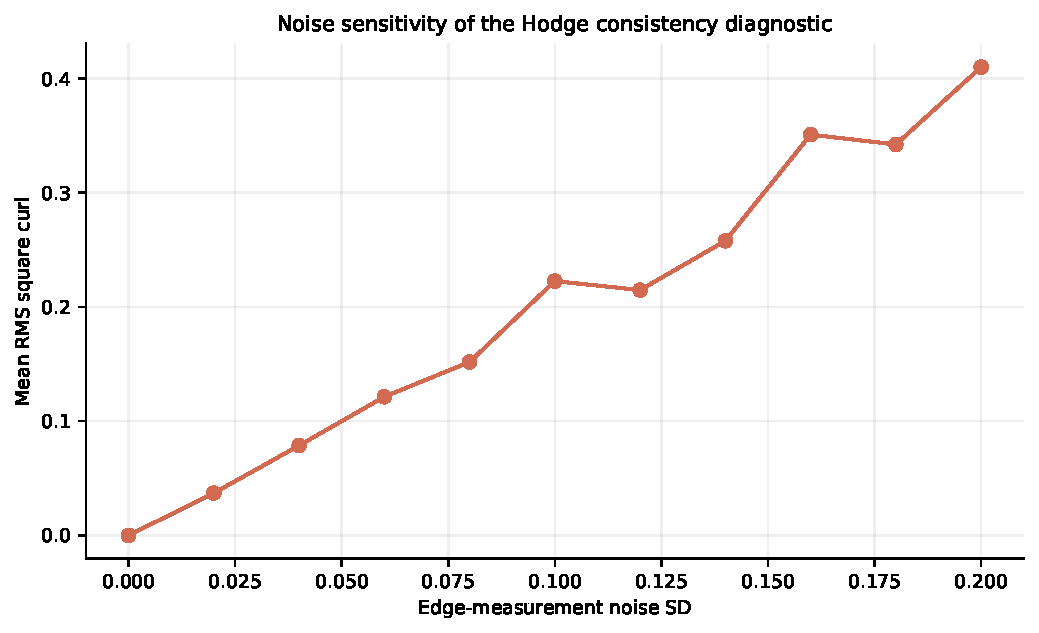
\includegraphics[width=0.82\linewidth]{figures/fig10_noise_sensitivity.pdf}\caption{Seeded sensitivity run for apparent square circulation under increasing independent edge-measurement noise. Each point averages RMS circulation over three synthetic landscapes; no empirical noise estimate is implied.}\label{fig:noise}\end{figure}

The initial conjecture stated that nonzero curl of drug-specific collateral-effect fields should decide whether an escape-proof schedule exists and lower-bound the number of drugs required. Under the scalar-potential interpretation, this cannot be correct as stated: the curl is zero before any policy is considered. Under an alternative definition of the field, nonzero curl may be meaningful, but its relationship to a safety guarantee must be established separately. This negative result prevents a topological analogy from being promoted into a theorem without a matching definition.

\section{Results II: robust viability and finite-horizon risk}
For the declared toy transition relation, the initial safe set contains 10 states. Greatest-fixed-point iteration reduces the candidate set through 6 states to a fixed kernel of 4 states. The kernel is $\{0000,0010,0100,0110\}$ under the bit convention in the script (integer states 0, 2, 4, and 6). Each retained state has at least one action whose entire successor set remains in the kernel. Thus the theorem's sufficient and necessary condition is directly verified for this finite benchmark. The starting state 0000 lies within the kernel.

The finite-horizon dynamic program gives zero probability of entering the synthetic failure set from state 0000 over the tested 12 steps under its optimizing action policy; this follows from this toy transition support, not a universal theorem about drugs. In independent 5,000-trajectory evaluations, the one-step greedy policy and round-robin policy enter the synthetic failure set frequently, while the trained tabular Q-learning policy also avoids it in this seeded run. Exact values are archived in \url{results/summary.json} and regenerated by \url{verify_model.py}. These rates are model outputs and must not be transported to another landscape, bacterial strain, drug panel, or dosing protocol.

\begin{figure}[htbp]\centering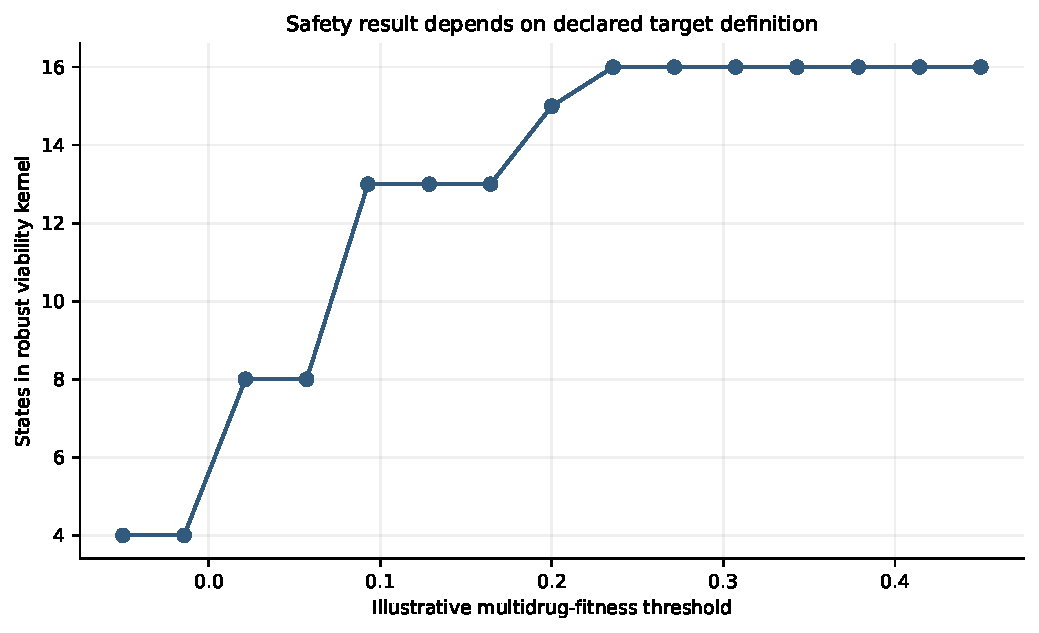
\includegraphics[width=0.80\linewidth]{figures/fig11_target_sensitivity.pdf}\caption{Robust-kernel size versus the illustrative threshold used to define the synthetic failure set. The plot emphasizes that safety conclusions are conditional on the operational definition of failure.}\label{fig:threshold}\end{figure}

\begin{table}[htbp]\centering\small\caption{Model-generated outputs for the declared synthetic benchmark.}\label{tab:results}\begin{tabularx}{\linewidth}{p{0.38\linewidth}p{0.20\linewidth}X}\toprule Quantity & Current run & Interpretation\\\midrule Genotypes / drugs & 16 / 3 & Four-locus toy hypercube; three action-specific landscapes.\\ Failure-set size & 6 & Set by the illustrative two-landscape threshold.\\ Robust viability kernel & 4 states & Exact for the selected successor relation.\\ Maximum exact square curl & $<1.2\times10^{-16}$ & Floating-point residual for scalar-potential differences.\\ Noisy edge-field RMS curl & 0.13--0.20 & Depends on seeded corruption and chosen scale.\\ Horizon-12 DP risk at 0000 & 0.000 & Synthetic finite-horizon kernel; not empirical.\\ Greedy / round-robin hit rate & 0.9926 / 0.9964 & Monte Carlo estimates, 5,000 trajectories each.\\ Q-learning hit rate & 0.0000 & One seeded training/evaluation configuration; not a safety proof.\\\bottomrule\end{tabularx}\end{table}

\section{Results III: threshold, noise, and model sensitivity}
The safety answer changes when the failure set changes. A stricter target may classify more states as unsafe and shrink the viability kernel; a more permissive target may enlarge it. Figure~\ref{fig:threshold} reports a threshold sweep with the transition relation held fixed. This is not parameter uncertainty in a resistance threshold; it demonstrates that a formal safety claim cannot be evaluated until the failure predicate is explicit. In real studies, the target requires phenotype criteria justified by organism, drug, assay, and clinical context.

The Hodge diagnostic has a different sensitivity profile. In the synthetic corruption experiment, independent edge noise tends to increase apparent cycle circulation. If noisy node fitness estimates are first fitted to a common scalar landscape and edge values are derived from those fitted nodes, the reconstructed field becomes exact by construction; uncertainty then appears in fitted potentials and residuals, rather than as independent edge curls. These are different analysis pipelines, and their results should not be mixed. A defensible empirical report should state whether the edge field was directly measured, computed from endpoint scores, or estimated jointly with a potential.

The model does not implement a neural surrogate for unseen genotypes or claim a large-genome scaling result. Such an extension would be meaningful only if it preserved held-out accuracy and calibrated uncertainty. An adversarial benchmark should compare an accurate model, an overconfident extrapolator, and a distribution shift in which mutational effects change outside training support. The relevant output is the probability that the claimed safe set contains actually unsafe states, not just prediction RMSE. This becomes important as the safety-game relation is widened to account for uncertainty.

\section{Competing explanations and falsification conditions}
Several alternative explanations could produce an observed nonzero circulation statistic in resistance data. First, measurements may have been collected under non-matching antibiotic concentrations or assay protocols. Second, edge effects may have been estimated independently, so measurement noise accumulates around cycles. Third, the chosen edges may not form a well-defined oriented complex, or some vertices may be missing. Fourth, observed quantities may be transition tendencies rather than differences in a shared scalar potential. Fifth, relevant state variables such as history, population composition, or environmental context may be omitted. These alternatives should be tested before interpreting circulation as intrinsic evolutionary dynamics.

Table~\ref{tab:falsify} defines practical falsification tests. The no-go proposition is an algebraic identity under its assumptions; an apparent counterexample would reveal a changed premise or an implementation error. The applied hypothesis that a Hodge statistic helps predict escape under real treatment landscapes requires out-of-sample predictive improvement over simpler baselines and a safety-game policy calibrated under uncertainty. A robust-policy claim is falsified if a biologically plausible transition leads from a supposedly safe state to the failure set while remaining consistent with the specified uncertainty set.

\begin{table}[htbp]\centering\small\caption{Falsification and diagnostic plan.}\label{tab:falsify}\begin{tabularx}{\linewidth}{p{0.27\linewidth}p{0.31\linewidth}X}\toprule Claim / failure mode & Test & Result that rejects the applied claim\\\midrule Static scalar-gradient curl & Recompute oriented cycle sums from common node potentials & Nonzero values beyond numerical tolerance imply inconsistent implementation or non-matching edge data.\\ Hodge statistic predicts escape & Held-out trajectory prediction against fitness-only baseline & No gain in calibrated prediction or decision utility.\\ Robust kernel is operationally safe & Validate allowed transitions and stress-test omitted edges & A plausible omitted transition reaches failure from a claimed safe state.\\ Q-learning generalizes & Independent landscapes, seeds, and parameter shifts & Performance collapses or safety violations remain frequent.\\ Neural landscape filling is reliable & Hold out genotypes and test uncertainty calibration & Overconfident unsafe predictions invalidate the certified relation.\\ History dependence is real & Compare matched genotypes across randomized drug histories & Transition difference disappears after controls or fails replication.\\\bottomrule\end{tabularx}\end{table}

\section{Polyhedral landscapes and alternative baselines}
Regular subdivisions and related polyhedral descriptions of fitness landscapes organize epistatic structure and genotype combinations under selection. These are complementary to the Hodge audit and safety game. A polyhedral representation summarizes geometry of a fitness function; it does not by itself answer which mutation transitions are feasible after each treatment or whether every allowed path can be prevented from entering a failure set. Conversely, the safety game can be solved from an explicit transition relation without a polyhedral construction. A meaningful comparison would ask whether polyhedral features predict the shape of viable regions or reduce the state space needed for exact planning, using the same held-out landscape instances and failure definition.

One baseline is the one-step greedy policy that chooses the drug with the lowest current synthetic fitness. It is locally intuitive but ignores long-run accessibility. Another is round-robin cycling; it is simple and reproducible but does not adapt to current state. The exact dynamic program is an oracle for its specified stochastic kernel and horizon, while the robust fixed-point computation is an oracle for the declared adversarial successor relation. Q-learning is an approximate learning baseline. Comparing them is valid only when objective, information, transition assumptions, initial-state distribution, and evaluation horizon are aligned. In this paper, the robust game and stochastic DP are reported as separate questions, not as interchangeable rankings.

\section{Toward empirical use: a staged validation protocol}
A real-data study would begin with a combinatorially complete landscape or an explicitly justified partial landscape for a small mutational system. Public TEM $\beta$-lactamase work provides a precedent for a landscape with 16 genotypes across 15 antibiotics, with later studies using those data for sequence optimization \citep{Mira2015,Nichol2015,Weaver2024}. In a new analysis, the data version, genotype encoding, assay conditions, and uncertainty estimates must be fixed before evaluating a Hodge-derived feature. This manuscript did not download or reanalyze those measurements; it uses them only as established context.

A conservative validation pipeline would have five stages. First, reconstruct node-level fitness distributions with replicate uncertainty and retain the exact genotype-environment mapping. Second, estimate uncertainty on edge contrasts and test cycle sums under a null model in which all edges derive from common node potentials. Third, define a phenotype-based failure set and state which transitions remain plausible under confidence bounds. Fourth, compute robust viability and finite-horizon risk under several defensible transition models, comparing against exact small-system solutions. Fifth, evaluate prediction and policy performance on held-out trajectories and report how often an allegedly safe policy violates its constraints under uncertainty expansion.

No human or animal intervention follows from this theoretical exercise. An eventual wet-lab investigation would need institutional biosafety review, organism- and assay-specific controls, antimicrobial stewardship oversight, and a protocol designed with qualified microbiology experts. Treatment schedules inferred in silico are not clinical prescriptions. The intended human benefit is indirect: better-calibrated tools for comparing evolutionary control strategies before costly or risky validation, if future empirical studies support them.

\section{Limitations and threats to validity}
The benchmark has deliberate limitations. Its 16 genotypes, three synthetic landscapes, threshold-defined failure set, and stylized beneficial-mutation kernel are far smaller and simpler than a real pathogen population. The model contains no recombination, horizontal gene transfer, demographic bottlenecks, spatial structure, phenotypic heterogeneity, persistence, immune response, pharmacokinetics, toxicity, or mixed infections. Its stochastic kernel is not an SSWM model calibrated to a known organism. The Monte Carlo outcomes demonstrate code behavior, not a biological fact.

The robust viability theorem is exact but conditional: an omitted successor invalidates the guarantee. Partial observation makes the problem harder because a belief state must account for all genotypes compatible with the data, and the number of beliefs can be exponential in genotype count. Hodge decompositions also depend on the complex selected for analysis. A graph without filled squares cannot reveal whether every cycle is a boundary; harmonic and coexact labels differ from those for the complete cube. The field's definition—fitness difference, transition log-odds, or another edge statistic—must be written down before interpretation.

Finally, “escape-proof” here means robust safety under a finite, specified relation. It is not a statement of clinical certainty. In open biological systems, an adversary model is incomplete and a finite landscape cannot enumerate all compensatory mutations. A practical goal is a transparent, uncertainty-aware risk bound with explicit scope rather than a promise of indefinite real-world prevention.

\section{Conclusion}
The proposed Hodge obstruction conjecture is not supported in its original form. If each drug's edge effect is a difference of a scalar fitness landscape, the resulting cochain is exact and every closed-loop circulation vanishes. Hodge decomposition can expose inconsistency in noisy or differently defined edge measurements, but no nonzero curl is available as a structural obstruction under this premise and no drug-count lower bound follows from it.

The existence of an escape-avoiding policy is instead characterized by the viability kernel of an explicit controlled transition relation. In a finite model, the greatest fixed point gives an exact robust safety guarantee, while a probabilistic dynamic program addresses finite-horizon risk under a specified kernel. The seeded synthetic benchmark verifies both computations, demonstrates sensitivity to the failure predicate, and separates exact mathematical identities from model-dependent outcomes. The next meaningful step is to define the measured edge field, quantify uncertainty, and test whether any Hodge-derived diagnostic improves held-out prediction or safety decisions beyond simpler landscape and transition models.

\section*{Research-process credit and disclosure}
Co-equal research-process credit is given to Devanik Debnath and Xylia, the autonomous multi-model research engine coordinating AI-assisted discovery, synthesis, and verification. Devanik Debnath retains responsibility for the final manuscript, scientific claims, citations, and released artifacts. AI assistance was used for literature synthesis, mathematical drafting, code construction, and verification planning; the author is responsible for checking the released work. This is a preprint and is not presented as peer-reviewed or clinically validated.
\label{maintext-end}\clearpage
\appendix
\section{Proof details for the cubical consistency identity}
For each locus pair $i<j$ and each base genotype $x$ whose bits $i$ and $j$ are zero, the oriented square has vertices $x$, $x+e_i$, $x+e_i+e_j$, and $x+e_j$. Its circulation is
\begin{equation}\label{eq:squareproof}\begin{aligned}&[f(x+e_i)-f(x)] + [f(x+e_i+e_j)-f(x+e_i)]\\&\quad + [f(x+e_j)-f(x+e_i+e_j)] + [f(x)-f(x+e_j)]=0.\end{aligned}\end{equation}
Every term cancels once with its opposite. Algebraically this is $B_2B_0=0$. The relation does not depend on the numerical values of $f$, so it holds for any real-valued potential. The released code uses least-squares projections to compute Hodge components and verifies that the exact field is reconstructed within numerical tolerance.

\section{Algorithms and computational complexity}
For $n=|V|$, $m=|\A|$, and $s=\max_{x,a}|\mathrm{Succ}(x,a)|$, one naive predecessor iteration costs $O(nms)$ after successor sets are built. There are at most $n$ strict elimination iterations, giving a simple upper bound $O(n^2ms)$; worklist-based algorithms may be faster on sparse systems. For horizon $H$, the dynamic program costs $O(Hmn^2)$ with dense transition matrices and less with sparse representations. Tabular Q-learning stores $nm$ action-values and updates one entry per observed transition. Exact belief-state enumeration can cost exponential time and memory, limiting use to small examples or carefully designed abstractions.

The safety and probability models must not be confused. The robust kernel uses only the support set of possible successors; it does not care whether an allowed successor is very unlikely. The stochastic dynamic program uses a probability distribution and minimizes expected hitting risk. In practical systems, it may be valuable to compute both: robust safety identifies states safe under all modeled possibilities, while the probabilistic calculation ranks policies when no robust solution exists or when a probabilistic objective is operationally accepted.

\section{Reproducibility instructions and data map}
All computations use Python 3.12-compatible syntax with NumPy, Matplotlib, and NetworkX. To regenerate numerical outputs, CSV data, and 12 numbered figure assets, run:
\begin{verbatim}python verify_model.py\end{verbatim}
The script fixes the landscape seed at 20261025, the Q-learning seed at 431, and separate seeds for Monte Carlo comparisons. It records actual package versions and check outcomes in \url{results/verification_report.json} and \url{results/verify_model_stdout.txt}. The figure inventory is in \url{results/figure_inventory.csv}; each data-bearing figure is generated by the same script and its underlying data are archived under \url{results/}.

The PDF is compiled from \url{paper.tex} and \url{paper.bib} by the clean-build helper in \url{deploy.py}, which invokes \texttt{latexmk} with fatal-error stopping enabled. The deployment script validates the root manifest and metadata, runs the verification script, and checks page/figure/table floors. These mechanics do not replace visual review of every rendered page. The visual-review record identifies the inspected PDF SHA-256, pages reviewed, defects, and disposition.

\section{Additional methodological notes}
The synthetic threshold is a formal predicate used to turn a continuous landscape into a reachability target. It is fixed in the current run and exposed through sensitivity analysis. The deterministic potential coefficients are disclosed in \url{verify_model.py} and are not fitted to real pathogen data. Their role is to generate a nontrivial test instance where landscape geometry and action choice can be inspected.

No public empirical records or external datasets were downloaded into the release. The literature audit records publication URLs and DOI metadata. Reanalysis of a public TEM landscape would be a separate phase requiring acquisition and versioning of original data tables, independent parsing, licensing review, and comparison against published benchmarks. That should precede any claim that this framework reproduces or outperforms an existing empirical treatment-sequence result.

\clearpage\bibliographystyle{plainnat}\bibliography{paper}
\end{document}
